

\section{Felsökning och felhantering}

Under arbete med portfolion kan fel uppstå på flera olika nivåer. Detta kapitel redogör för vilka metoder och verktyg man kan använda för att undersöka och åtgärda vanliga fel.

Generellt för all felsökning är att det är bra att spara och testa kodens funktion ofta. Om man ändrar en liten del av koden, och det sedan inte fungerar, är det mycket lättare att hitta nyss implementerade fel. Om man däremot har ändrat stora delar av koden utan att kontinuerligt testa, kan felet i princip ligga var som helst, och det kan bli mycket svårare att hitta det.


\subsection{Felsökning med hjälp av Flask}
Under utvecklingen kan fel uppstå i Python-koden eller i Jinja2-templaten som gör att sidan inte kan visas. Förutom syntaxfel i Python-koden, som behandlas nedan, kommer man inte att få ett felmeddelande i terminalfönstret. Istället visas inte sidan när man försöker ladda den. Om man kör appen i vanligt läge kommer sidan att visa ''Internal Server Error''. Under utvecklingsarbetet kan man dock använda debug-läge för att få mer information om felet. Debug-läge aktiveras vid att skicka detta som parameter till run-funktionen i myFlaskProject.py:

\begin{figure}
  \centering
  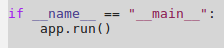
\includegraphics{debugmode}
  \caption{Kod längst ner i myFlaskProject.py för att aktivera debug-läge}
\end{figure}


Fördelen med att använda debugläge är dels att servern automatiskt startas om när man sparar ändringar i en fil, samt att man istället för sidan ''Internal Server Error'' får upp en detaljerad logg över senaste utförda kodrader och en beskrivning av felet.
Debugläget visar information om fel som uppstår både i myFlaskProject.py och i Jinja2-templat.

\textbf{Notera:} Flasks debug-läge ska inte användas på en server som ligger tillgänglig online, då detta utgör en säkerhetsrisk.

\begin{figure}
  \centering
  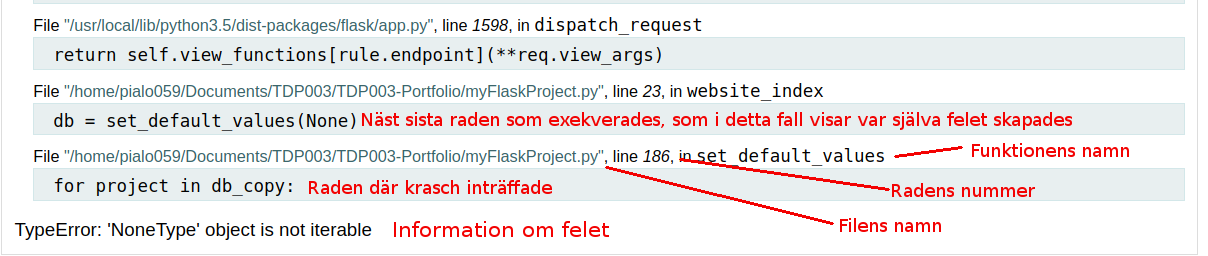
\includegraphics{flaskdebug1}
  \caption{Debuggerns utseende vid fel i myFlaskProject.py. Användbar information är filens namn, exekverade kommandon, radnummer och namn på funktion, samt beskrivning av felet}
\end{figure}

\begin{figure}
  \centering
  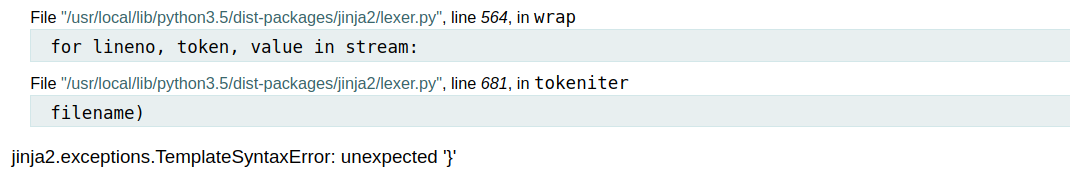
\includegraphics{flaskdebug2}
  \caption{Debuggerns utseende vid fel i ett Jinja2-templat. Användbar information är beskrivning av felet.}
\end{figure}
  

\subsection{Felsökning av Python-kod}
Om utvecklaren inför syntaxfel i Python-koden startar inte servern. Alternativt, om servern har startats i debug-läge, som förklarat ovan, kommer servern att stoppas. Vid omladdning av sidan får man då upp att sidan inte kan nås.
Terminalfönstret innehållar då information om felet, och man kan använda denna information för att hitta var i koden felet har uppstått.

\begin{figure}
  \centering
  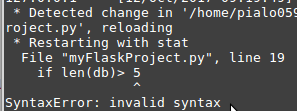
\includegraphics{python_error}
  \caption{Terminalfönstrets utseende vid ett syntaxfel i myFlaskProject.py. Felbeskrivningen innehåller namn på filen, radnummer där felet uppstod, raden som förde till kraschet och en pil som ofta visar exakt var felet ligger i raden}
\end{figure}

\subsection{Felaktigt utseende}
Om sidan laddar, men inte ser ut som förväntat, är det troligt att det finns ett fel i HTML-templatet för sidan. Vid testning i Chrome kan man använda Chromes utvecklarverktyg för att undersöka sidans struktur närmre. Två av dessa verktyg är särskilt till hjälp.

\subsubsection{Sidans källkod}
För att komma åt sidans källkod, högerklicka på sidan och välj ''View page sourse''. Alternativt kan man på en PC klicka Ctrl + U. På sidans källkod kan man hitta den genererade HTML-koden. Detta är till hjälp om man till exempel vill kolla att externa länkar och länkar till filnamn har genererats rätt.

\begin{figure}
  \centering
  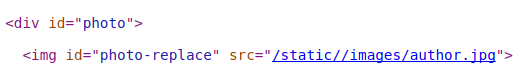
\includegraphics{sourcecode}
  \caption{Fel i genererad bildadress i källkoden}
\end{figure}


\subsubsection{Inspektera HTML-element}
Vid att högerklicka på ett element och välja ''Inspect'' kan man undersöka HTML-kod och CSS för olika sidelement. Detta är ett myket bra verktyg för att felsöka fel i elements utseende, och det kan användas på flera olika sätt. Olika möjligheter i detta verktyg inkluderar:

\begin{itemize}
\item: Se vilka delar av sidan som ingår i olika HTML-element - Underlättar att se fel i placering av taggar för att öppna och stänga element
\item: Se boxmodell av elementet - Underlättar att se fel i storlekar på olika delar (height, width, padding, margin) av elementet.
\item: Se CSS-egenskaper som berör elementet - Underlättar att se om en CSS-egenskap överskrivs av samma CSS-egenskap i en annan klass
\item: Ändra CSS-egenskaper - Möjliggör snabb testning av ändringar av olika egenskaper
\end{item}


\begin{figure}
  \centering
  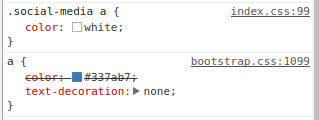
\includegraphics{inspectelement}
  \caption{Undersökning av CSS-egenskaper i inspektion av element. Här kan man se att a-elementets färg skulle varit #337ab7 enligt bootstrap.css-filen, men att deta har överskrivits i filen index.css
\end{figure}


\subsection{Felsökning i OpenShift}
Vid uppladdning av portfolion i OpenShift kan olika problem uppstå. OpenShift Client Tools, rhc, inkluderar loggfiler där man kan få information om olika fel som har uppstått. Man kan komma åt en utskrift av de senaste loggar med kommandot \texttt{rhc tail -a appnamn}. Information man kan få från detta verktyg inkluderar problem med att komma åt olika moduler i appen, samt problem med att öppna filer på grund av teckenkodning.
